\documentclass[a4paper,11pt]{article}

%% We can use macros to avoid typing the same thing over and over
\newcommand{\token}[1]{\texttt{<#1>}}
\newcommand{\uC}{{$\mathrm{\mu}$}C }
 \usepackage{tikz}
 \usepackage{tikz-qtree}
 \usepackage{array}
\usepackage{amsmath}
\usepackage{multicol}

\title{Assignment 2: Parser}
\author{Xiao Yang \and Magnus L{\aa}ng} % replace by your name(s)
\date{\today}
\begin{document}
\maketitle

\section{Technical Issues}
For building the AST in the parser, we use the JJTree tool which is part of the JavaCC distribution.
JJTree builds the AST bottom-up using a stack of nodes, taking an annotated JavaCC grammar as input and generating a pure JavaCC parser with tree building code inserted.
Productions can be annotated to not envelop everything on their ``stack frame'' in a node of their own, but rather just pass the nodes along to the next level up, allowing us to build ASTs using JJTree.
Also, annotations that pops a certain number of nodes and makes a new node of them can be inserted at any position within a production.

\subsection{Precedence of Binary Operators}
When we rewrite the grammar to remove ambiguity and enforce the precedence of operators, we expand the expression production into a chain of productions.
The production with the lowest precedence operators become the starting production for an expression, which then produces non-terminals of the next precendence level, and so on.

For example, a grammar of addition and multiplication could express the higher precendence of multiplication in the following way:
\begin{align*}
  Expr \rightarrow &\; Expr \;\text{``\texttt{+}''}\; Expr' \\
       \mid \:     &\; Expr'
\end{align*}
\begin{align*}
  Expr' \rightarrow &\; Expr' \;\text{``\texttt{*}''}\; Expr'' \\
        \mid \:     &\; Expr''
\end{align*}

\subsection{Associativity of Binary Operators}
\begin{itemize}
	\item \textbf{Left-Associative} \\
	For left-associative operators, we use \emph{EBNF} to rewrite the grammar.
	Taking expressions with addition as an example, we write the following grammar rule:
	\begin{equation*}
		Expr \rightarrow Expr' \;(\text{``\texttt{+}''}\; Expr' \;\dag)^*
	\end{equation*}

    We annotate the grammar at {\dag} that JJTree should pop two nodes off of the stack, and add them to a \emph{Binary} node.
    Note that if the Kleene-star is expanded several times, the left-hand side node that is popped off the stack will not be the node generated by $Expr'$, but rather the \emph{Binary} node generated by the previous expansion of the Kleene-star.
    This means the tree will be built in left-associative form.

	\item \textbf{Right-Associative} \\
	For right-associative operators, we adopt right-recursive rules to build the corresponding nodes.
	Taking assignment as an example, we write the following rule:
	\begin{align*}
		Expr \rightarrow &\; Expr' \;\text{``\texttt{=}''}\; Expr \\
             \mid \:     &\; Expr'
	\end{align*}
\end{itemize}


\newpage
\appendix
\renewcommand\thesection{Appendix \Alph{section}} %% Add the word ``Appendix'' to the numbering

\section{AST Structure}
Here we present the nodes and their children of our Abstract Syntax Tree. Note that \emph{\#Expression} and \emph{\#Statement} are abstract node classes which are used to ease the representaion of the tree structure. The real nodes belong to these two classes are listed in the end.

\hspace{1em}

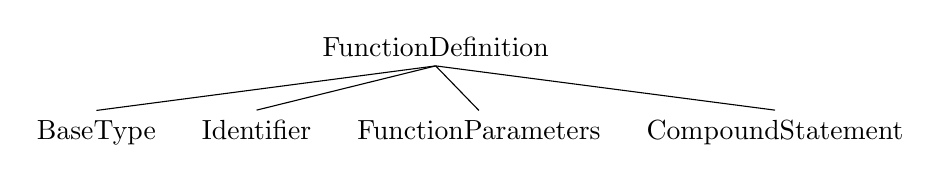
\begin{tikzpicture}[grow=down]
\tikzset{level distance = 30pt, sibling distance = 10pt}

\Tree [.FunctionDefinition
			[.BaseType ]
			[.Identifier ]
			[.FunctionParameters ]
			[.CompoundStatement ]
		]

\end{tikzpicture}

\hspace{1em}

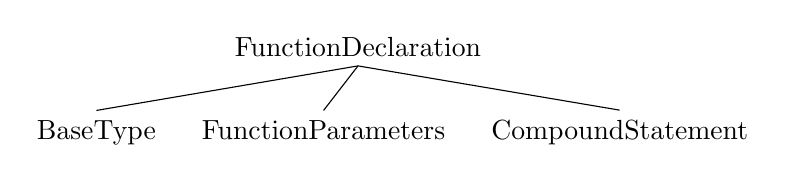
\begin{tikzpicture}[grow=down]
\tikzset{level distance = 30pt, sibling distance = 10pt}

\Tree [.FunctionDeclaration
			[.BaseType ]
			[.FunctionParameters ]
			[.CompoundStatement ]
		]

\end{tikzpicture}

\hspace{1em}

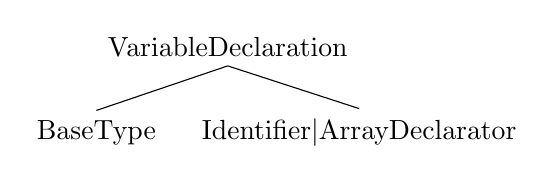
\begin{tikzpicture}[grow=down]
\tikzset{level distance = 30pt, sibling distance = 10pt}

\Tree [.VariableDeclaration
			[.BaseType ]
			[.Identifier$|$ArrayDeclarator ]
		]

\end{tikzpicture}

\hspace{1em}

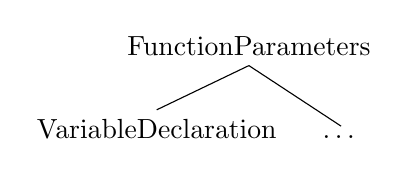
\begin{tikzpicture}[grow=down]
\tikzset{level distance = 30pt, sibling distance = 10pt}

\Tree [.FunctionParameters
			[.VariableDeclaration ]
			[.$\dots$ ]
		]

\end{tikzpicture}

\hspace{1em}

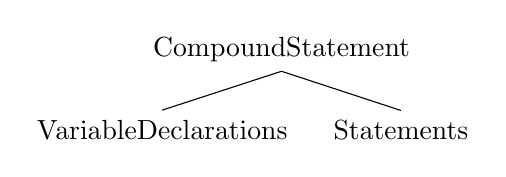
\begin{tikzpicture}[grow=down]
\tikzset{level distance = 30pt, sibling distance = 10pt}

\Tree [.CompoundStatement
			[.VariableDeclarations ]
			[.Statements ]
		]

\end{tikzpicture}

\hspace{1em}

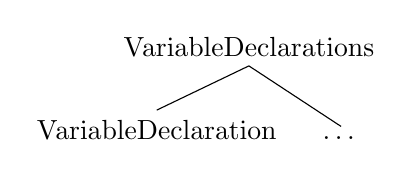
\begin{tikzpicture}[grow=down]
\tikzset{level distance = 30pt, sibling distance = 10pt}

\Tree [.VariableDeclarations
			[.VariableDeclaration ]
			[.$\dots$ ]
		]

\end{tikzpicture}

\hspace{1em}

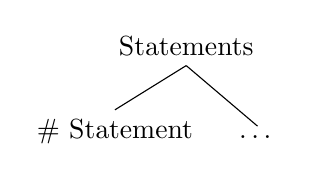
\begin{tikzpicture}[grow=down]
\tikzset{level distance = 30pt, sibling distance = 10pt}

\Tree [.Statements
			[.\#~Statement ]
			[.$\dots$ ]
		]

\end{tikzpicture}

\hspace{1em}

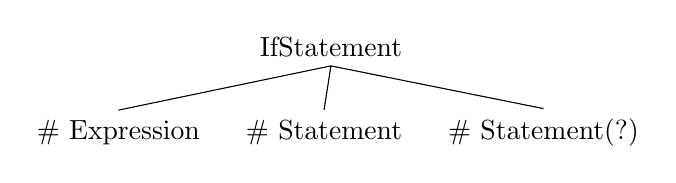
\begin{tikzpicture}[grow=down]
\tikzset{level distance = 30pt, sibling distance = 10pt}

\Tree [.IfStatement
			[.\#~Expression ]
			[.\#~Statement ]
			[.\#~Statement(?) ]
		]
\end{tikzpicture}

\hspace{1em}

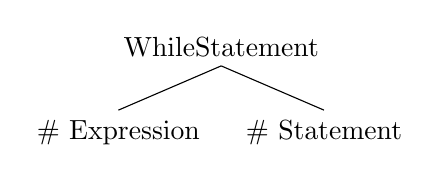
\begin{tikzpicture}[grow=down]
\tikzset{level distance = 30pt, sibling distance = 10pt}
\Tree [.WhileStatement
			[.\#~Expression ]
			[.\#~Statement ]
		]
\end{tikzpicture}

\hspace{1em}

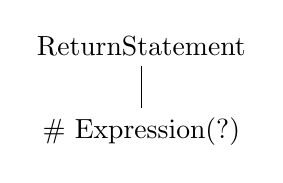
\begin{tikzpicture}[grow=down]
\tikzset{level distance = 30pt, sibling distance = 10pt}
\Tree [.ReturnStatement
			[.\#~Expression(?) ]
		]
\end{tikzpicture}

\hspace{1em}

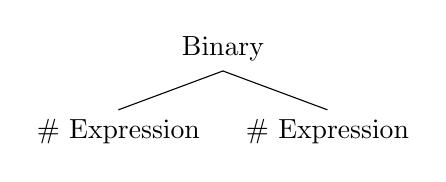
\begin{tikzpicture}[grow=down]
\tikzset{level distance = 30pt, sibling distance = 10pt}
\Tree [.Binary
			[.\#~Expression ]
			[.\#~Expression ]
		]
\end{tikzpicture}

\hspace{1em}

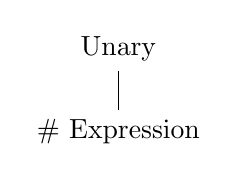
\begin{tikzpicture}[grow=down]
\tikzset{level distance = 30pt, sibling distance = 10pt}
\Tree [.Unary
			[.\#~Expression ]
		]
\end{tikzpicture}

\hspace{1em}

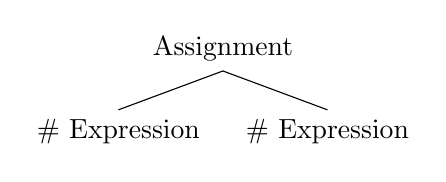
\begin{tikzpicture}[grow=down]
\tikzset{level distance = 30pt, sibling distance = 10pt}
\Tree [.Assignment
			[.\#~Expression ]
			[.\#~Expression ]
		]
\end{tikzpicture}

\hspace{1em}

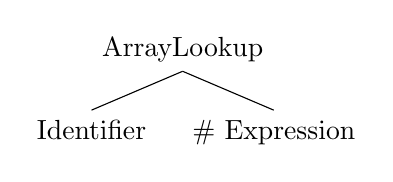
\begin{tikzpicture}[grow=down]
\tikzset{level distance = 30pt, sibling distance = 10pt}
\Tree [.ArrayLookup
			[.Identifier ]
			[.\#~Expression ]
		]
\end{tikzpicture}


\begin{multicols}{2}
\paragraph{\#~Statement}
\begin{itemize}
	\item IfStatement
	\item EmptyStatement
	\item WhileStatement
	\item CompoundStatement
	\item ReturnStatement
	\item \#~Expression
\end{itemize}

\paragraph{\#~Expression}
\begin{itemize}
	\item Binary
	\item Assignment
	\item Unary
	\item IntegerLiteral
	\item Identifier
	\item ArrayLookup
\end{itemize}
\end{multicols}

\end{document}
